\textbf{Задание №8} «Путешествие виртуального адреса». Разработать программу, которая получает несколько
виртуальных адресов: функции программы, глобальной переменной, локальной переменной,
объекта malloc() и области mmap(). Для каждой страницы программа должна вычислить номер
виртуальной страницы и смещение внутри неё. Для архитектуры x86-64 и стандартной
страницы 4 КБ дополнительно разложить виртуальный адрес на поля PML4, PDPT, PD, PT и
offset; при поддержке пятиуровневой адресации предусмотреть вывод дополнительного индекса
PML5. Затем выполнить обход большого массива с шагом 64 байта, 4 КБ, 16 КБ и 64 КБ и
сравнить dTLB-load-misses. Пояснить различие между TLB miss, page table walk и page fault \label{sec:8}

\begin{minted}[frame=lines, framesep=2mm, baselinestretch=1.2, fontsize=\small, linenos]{c}
#define _GNU_SOURCE
#include <stdio.h>
#include <stdlib.h>
#include <stdint.h>
#include <string.h>
#include <unistd.h>
#include <time.h>
#include <sys/mman.h>
#include <sys/ioctl.h>
#include <sys/syscall.h>
#include <linux/perf_event.h>

void show(uint64_t a, const char *name, int has_la57)
{
    printf("%s\n", name);
    printf("  Адрес:                  0x%016lx\n", a);
    uint64_t vpn = a >> 12;
    uint64_t off = a & 0xFFF;
    printf("  VPN: %lu (0x%lx),  offset: %lu (0x%lx)\n",
           vpn, vpn, off, off);
    if (has_la57)
        printf("  PML5=%lu  ", (a >> 48) & 0x1FF);
    else
        printf("  PML5=0  ");
    printf("PML4=%lu  PDPT=%lu  PD=%lu  PT=%lu\n",
           (a >> 39) & 0x1FF, (a >> 30) & 0x1FF,
           (a >> 21) & 0x1FF, (a >> 12) & 0x1FF);
    printf("\n");
}

void show_all(int has_la57)
{
    static int g_data = 42;
    static int g_bss;
    int loc = 7;
    void *h = malloc(4096);
    void *m = mmap(NULL, 4096, PROT_READ | PROT_WRITE,
                   MAP_PRIVATE | MAP_ANONYMOUS, -1, 0);

    struct { uint64_t addr; const char *name; } items[] = {
        { (uint64_t)&main,   "main()        (.text)" },
        { (uint64_t)&g_data, "static local  (.data)" },
        { (uint64_t)&g_bss,  "static local  (.bss) " },
        { (uint64_t)&loc,    "auto local    (stack)" },
        { (uint64_t)h,       "malloc        (heap) " },
        { (uint64_t)m,       "mmap          (anon) " },
    };

    for (size_t i = 0; i < sizeof(items) / sizeof(items[0]); i++)
        show(items[i].addr, items[i].name, has_la57);

    free(h);
    munmap(m, 4096);
}

int perf_open(void)
{
    struct perf_event_attr pe = {
        .type   = PERF_TYPE_HW_CACHE,
        .size   = sizeof(pe),
        .config = PERF_COUNT_HW_CACHE_DTLB
                | (PERF_COUNT_HW_CACHE_OP_READ     << 8)
                | (PERF_COUNT_HW_CACHE_RESULT_MISS << 16),
        .disabled = 1, .exclude_kernel = 1, .exclude_hv = 1,
    };
    return (int)syscall(__NR_perf_event_open, &pe, 0, -1, -1, 0);
}

long long bench(unsigned char *a, size_t sz, size_t step)
{
    int fd = perf_open();
    long long miss = -1;
    if (fd >= 0) {
        ioctl(fd, PERF_EVENT_IOC_RESET,  0);
        ioctl(fd, PERF_EVENT_IOC_ENABLE, 0);
    }

    struct timespec t0, t1;
    clock_gettime(CLOCK_MONOTONIC, &t0);
    volatile unsigned char s = 0;
    for (size_t i = 0; i < sz; i += step) s += a[i];
    clock_gettime(CLOCK_MONOTONIC, &t1);

    if (fd >= 0) {
        ioctl(fd, PERF_EVENT_IOC_DISABLE, 0);
        read(fd, &miss, sizeof(miss));
        close(fd);
    }

    double dt = (t1.tv_sec - t0.tv_sec) + (t1.tv_nsec - t0.tv_nsec) / 1e9;

    size_t reads      = sz / step;
    double mb_read    = (double)reads / (1024.0 * 1024.0);
    double read_speed = mb_read / dt;                
    double miss_rate  = (miss >= 0)
                      ? 100.0 * (double)miss / (double)reads
                      : -1.0;

    printf("step = %6zu B : t = %.6f s, reads = %8zu, "
           "read = %7.3f MB, speed = %10.1f MB/s, "
           "dTLB-misses = %lld",
           step, dt, reads, mb_read, read_speed, miss);
    if (miss_rate >= 0.0)
        printf("  (%.1f%% от reads)", miss_rate);
    printf("\n");

    (void)s;
    return miss;
}

int detect_la57(void)
{
    FILE *f = fopen("/proc/cpuinfo", "r");
    if (!f) return 0;
    char line[512];
    int r = 0;
    while (fgets(line, sizeof(line), f))
        if (strstr(line, "la57")) { r = 1; break; }
    fclose(f);
    return r;
}

int main(void)
{
    setvbuf(stdout, NULL, _IONBF, 0);

    int has_la57 = detect_la57();
    printf("Размер страницы: %ld байт\n", sysconf(_SC_PAGESIZE));
    printf("LA57 (5 уровней): %s\n\n", has_la57 ? "да" : "нет");

    show_all(has_la57);

    size_t sz = 64UL << 20;
    unsigned char *a = mmap(NULL, sz, PROT_READ | PROT_WRITE,
                            MAP_PRIVATE | MAP_ANONYMOUS, -1, 0);
    if (a == MAP_FAILED) { perror("mmap"); return 1; }
    memset(a, 1, sz);

    printf("Обход массива 64 МБ\n");
    long long m64  = bench(a, sz,    64);
    long long m4k  = bench(a, sz,  4096);
    long long m16  = bench(a, sz, 16384);
    long long m64k = bench(a, sz, 65536);

    munmap(a, sz);

    printf("\nСравнение dTLB-misses:\n");
    printf("  step =    64 B : %lld\n", m64);
    printf("  step =  4096 B : %lld\n", m4k);
    printf("  step = 16384 B : %lld\n", m16);
    printf("  step = 65536 B : %lld\n", m64k);
    if (m64k > 0)
        printf("  Отношение 64 B / 64 KB = %.2f\n",
               (double)m64 / (double)m64k);

    return 0;
}
\end{minted}

\begin{figure}[H]
    \centering
    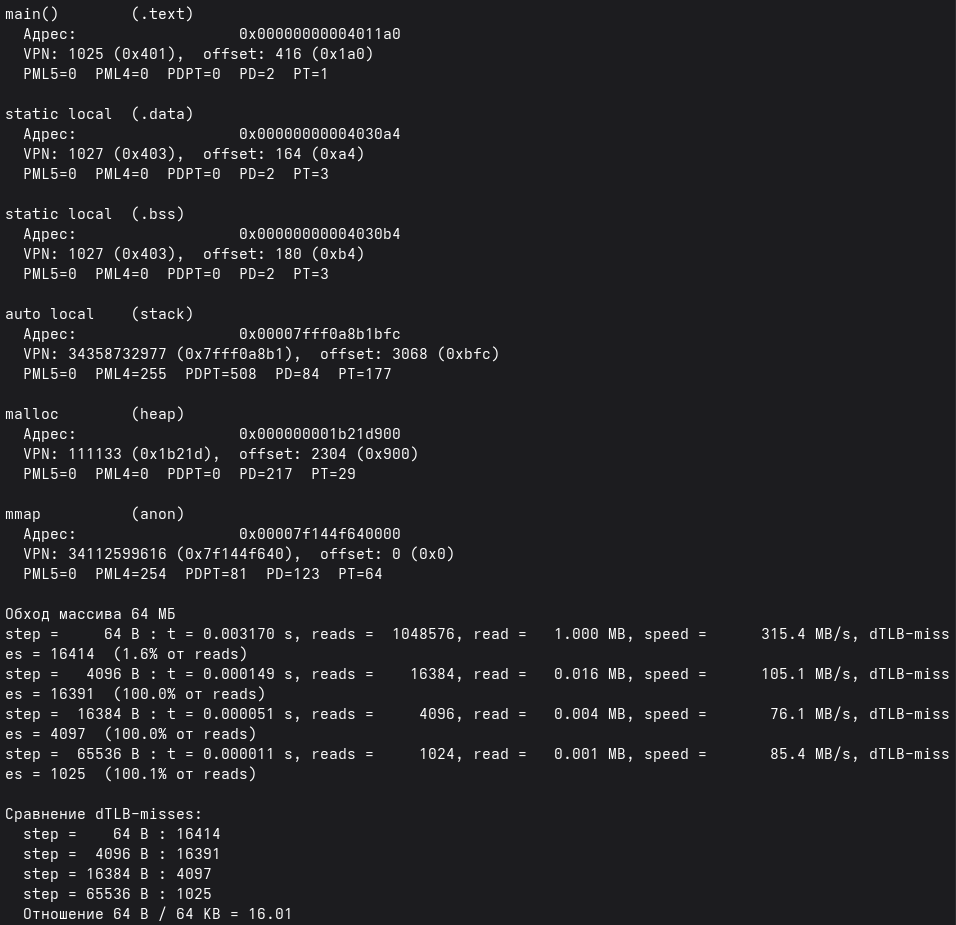
\includegraphics[width = 1 \textwidth]{picture/res.png}
    \caption{Результат выполнения программы}
\end{figure}

Программа демонстрирует структуру виртуального адреса в архитектуре
x86-64 и исследует влияние шага обхода массива на промахи TLB
(Translation Lookaside Buffer).

\begin{enumerate}
\item Что делает программа

\begin{enumerate}
    \item \textbf{Определяет характеристики системы:}
    \begin{enumerate}
        \item размер страницы через \texttt{sysconf(\_SC\_PAGESIZE)};
        \item поддержку пятиуровневой адресации LA57 через анализ
        \texttt{/proc/cpuinfo}.
    \end{enumerate}
    
    \item \textbf{Получает шесть виртуальных адресов:}
    \begin{enumerate}
        \item функции \texttt{main} (\texttt{.text});
        \item инициализированной статической переменной (\texttt{.data});
        \item неинициализированной статической переменной (\texttt{.bss});
        \item локальной переменной (\texttt{stack});
        \item объекта \texttt{malloc(4096)} (\texttt{heap}, через \texttt{brk});
        \item области \texttt{mmap()} (анонимное отображение).
    \end{enumerate}
    
    \item \textbf{Для каждого адреса вычисляет:}
    \begin{enumerate}
        \item номер виртуальной страницы (VPN): \texttt{a >> 12};
        \item смещение внутри страницы: \texttt{a \& 0xFFF};
        \item поля таблицы страниц:
        \begin{enumerate}
            \item \texttt{PML5} — биты 48--56 (только при LA57);
            \item \texttt{PML4} — биты 39--47;
            \item \texttt{PDPT} — биты 30--38;
            \item \texttt{PD} — биты 21--29;
            \item \texttt{PT} — биты 12--20.
        \end{enumerate}
    \end{enumerate}
    
    \item \textbf{Выполняет обход массива 64~МБ} с шагами 64~Б, 4~КБ,
    16~КБ и 64~КБ. Для каждого шага измеряет:
    \begin{enumerate}
        \item время обхода;
        \item количество реально прочитанных байт;
        \item скорость чтения;
        \item количество промахов \texttt{dTLB-load-misses} через
        \texttt{perf\_event\_open};
        \item долю промахов от числа обращений (miss rate).
    \end{enumerate}
    
    \item \textbf{Сравнивает} полученные значения dTLB-misses между
    всеми шагами и вычисляет отношение 64~Б / 64~КБ.
\end{enumerate}

\item Использованные средства

\begin{center}
\begin{tabular}{ll}
\toprule
\textbf{Средство} & \textbf{Назначение} \\
\midrule
\texttt{sysconf} & размер страницы \\
\texttt{fopen}/\texttt{fgets} & чтение \texttt{/proc/cpuinfo} \\
\texttt{mmap} & выделение массива 64~МБ \\
\texttt{memset} & инициализация массива \\
\texttt{malloc}/\texttt{free} & heap-объект \\
\texttt{perf\_event\_open} & счётчик dTLB-load-misses \\
\texttt{ioctl} & управление perf-счётчиком \\
\texttt{clock\_gettime} & замер времени \\
\texttt{printf} & вывод результатов \\
\bottomrule
\end{tabular}
\end{center}

\item Что демонстрирует

\begin{enumerate}
    \item \textbf{Адреса разных сегментов лежат в разных VMA:}
    \begin{enumerate}
        \item \texttt{.text}/\texttt{.data}/\texttt{.bss} — низкие адреса
        \texttt{0x40\ldots}, \texttt{PML4 = 0};
        \item \texttt{malloc} — heap (\texttt{brk}), тоже \texttt{PML4 = 0};
        \item \texttt{stack} — \texttt{0x7fff\ldots}, \texttt{PML4 = 255};
        \item \texttt{mmap} — \texttt{0x7f\ldots}, \texttt{PML4 = 254}.
    \end{enumerate}
    
    \item \textbf{Поля таблицы страниц} корректно разлагают адрес на
    индексы и смещение.
    
    \item \textbf{Абсолютное число dTLB-misses пропорционально числу
    страниц}, а не числу обращений:
    \begin{enumerate}
        \item шаг 64~Б: $\sim$1.6\% промахов (63 из 64 обращений —
        попадание в TLB);
        \item шаг $\ge$ 4~КБ: $\sim$100\% промахов (каждое обращение —
        новая страница).
    \end{enumerate}
    
    \item \textbf{Отношение dTLB-misses 64~Б / 64~КБ $\approx$ 16}
    совпадает с отношением числа страниц (16384 / 1024 = 16).
    
    \item \textbf{TLB miss $\ne$ page fault:} page fault не возникало,
    все промахи обрабатывались аппаратно (page table walk).
\end{enumerate}
\end{enumerate}